
%%%%%%%%%%%%%%%%%%%%%%%%%%%%%%%%%%%%%%%%%%%%%%%%%%%%%%%%%%%%%%%%%%%%%%%%%%%%%%%%%%%%%%%%%%%%%%%%%%%%%%%
% Sequence Homology Search}
%%%%%%%%%%%%%%%%%%%%%%%%%%%%%%%%%%%%%%%%%%%%%%%%%%%%%%%%%%%%%%%%%%%%%%%%%%%%%%%%%%%%%%%%%%%%%%%%%%%%%%%

\fancychapter{Sequence Homology Search}

This chapter will present two of the most widely used methods to search for homolog sequences: Alignment Algorithms described in the first section; and probabilistic models known as Markov Models, presented in the second section.


%%%%%%%%%%%%%%%%%%%%%%%%%%%%%%%%%%%%%%%%%%%%%%%%%%%%%%%%%%%%%%%%%%%%%%%%%%%%%%%%%%%%%%%%%%%%%%%%%%%%%%%
%%%%%%%%%%%%%%%%%%%%%%%%%%%%%%%%%%%%%%%%%%%%%%%%%%%%%%%%%%%%%%%%%%%%%%%%%%%%%%%%%%%%%%%%%%%%%%%%%%%%%%%

\section{Alignment Algorithms}

Sequence alignment is a very simple technique: taking two sequences, aligning its symbols side by side, \emph{in order}, and inserting gaps to fill the places of inserted or deleted symbols (a deletion in one sequence is equivalent to an insertion in the other). An alignment of two sequences can be easily extracted from an edit distance matrix, and it shows in a very readable form the divergences between the two sequences, as well as the matches between them (known in molecular biology as 'conserved regions').

As such, the alignment of two protein or DNA strings is a useful and appealing way of highlighting their similarity. More than that, the aligning procedure serves the goal of evaluating and quantifying how interesting is the alignment found; or in other words, how related or distant are the sequences. For these reasons, it became the main technique used to study protein and DNA mutations.

The alignment can be global, in which the whole sequences are aligned, from start to finish; or it can be local, aligning only a certain, partial region of each sequence. The algorithms described in the next sections are 'optimal' algorithms - they are guaranteed to find the best possible alignment according to a specific distance (homology) metric. Later on, some non-optimal (i.e. heuristic) alignment algorithms will be briefly presented.

To measure the performance of alignment programs, the CUP measure is the most widely used. CUP stands for 'Cell Update per Second', though a more suitable name would be 'Cell Computation per Second'. The final CUP score for one single alignment is given by $\frac{M \times N}{t}$, where M and N are the sequences' lengths, and t is time in seconds. Since the CUP scores in modern processors and implementations are very high, MCPs (mega CUPs) and GCUPs (giga CUPs) are more common.



\subsection{Edit Distance of Levenshtein}

%It is commonly known simply as 'edit distance', since it has become the ubiquitous metric for approximate string comparison, extensively used in the areas of Information Indexing and Retrieval, Text Processing, Automatic Spellchecking; besides numerous applications in other areas.

A good starting point is the popular 'Edit Distance', first formulated by Levenshtein in 1966 \cite{levenshtein} for string matching. The edit distance of two sequences is defined as the minimum number of edit operations necessary to transform one sequence into the other. An edit operation may be a substitution, an insertion of a symbol, or a deletion of a symbol (the insertion of a symbol from sequence A in sequence B can always be replaced by the deletion of that symbol in sequence A, hence these last two operations are symmetrical). Insertions and deletions (indels) are usually referred to as 'insertions of gaps' in the context of biological alignments.

The levenshtein edit distance if usually computed with resort to an also well-known Dynamic Programming algorithm, first defined by Wagner and Fischer in 1974 \cite{wagner1974string}. It uses a typical \ac{DP} matrix to map the three dependencies of the algorithm: match of the two symbols or substitution of one symbol for the other, deletion of a symbol from a sequence, or insertion into that sequence. In matches and substitutions, both symbols are consumed and the algorithm moves to the next cell in the diagonal. In insertions and deletions, only one symbol is consumed from one of sequences. Each cell computes a function given by the Maximum or Minimum of its dependencies' costs (diagonal, horizontal and vertical), and chooses the origin (dependency) that has the best cost and so yields the best result for that cell. This algorithm, and all similar ones, have quadratic complexity $O(n  \times  m)$, since it requires the computation of all $N \times M$ matrix cells.

The edit distance recursive relation can be formulated as follows:
\hspace{1 pc} $$D_{m,n} = Min \hspace{0.2cm}(D_{m-1,n-1} + SubstScore, \hspace{0.2cm} D_{m,n-1} + GapCost, \hspace{0.2cm}  D_{m-1,n} + GapCost ) $$
where the value of SubstScore depends on whether it is a match or mismatch. An example is presented in \autoref{edit-distance} and \autoref{alignments}, with a match score of 0 and mismatch of 1.

The optimal alignment of the two sequences can be easily extracted from the Edit Distance matrix, using a tracebacking mechanism. The procedure starts from the last cell, and traces each choice of the algorithm (i.e. the path chosen for each cell) until the starting point. In order to do this, each cell must keep the dependency (direction) used to compute its own value. 
%which of the three dependencies was used to compute its own value.


\begin{figure}[htb!]
  \begin{minipage}{0.48\linewidth}
	\centering
	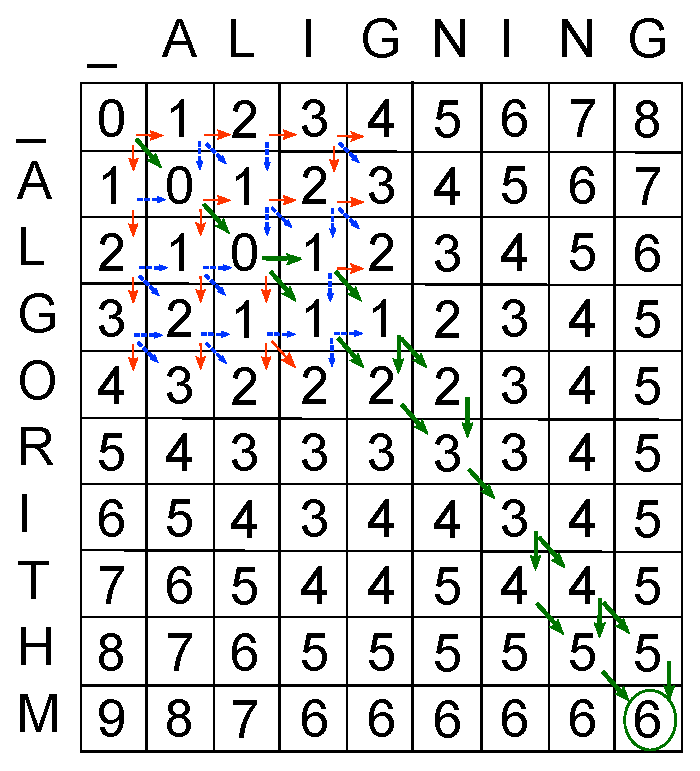
\includegraphics[scale=0.6]{img-align/edit-distance.eps}
	\caption[Edit Distance alignment] {Edit Distance matrix for sequences 'algorithm' and 'aligning', using unitary costs. The first dependencies are marked. The non-picked directions have dotted blue lines, picked ones are red and straight, and the optimal path is in green bold.}
	\label{edit-distance}
  \end{minipage}
  \hspace{0.04\linewidth}
  \begin{minipage}{0.48\linewidth}
	\centering
	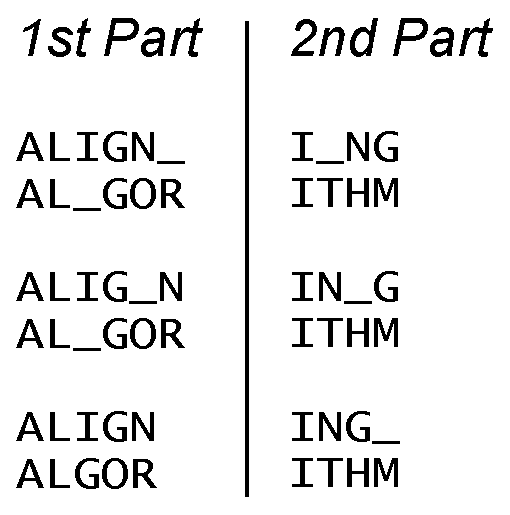
\includegraphics[scale=0.5]{img-align/alignments.eps}
	\caption[Resulting optimal alignments from Edit Distance]{Resulting 9 optimal alignments - each part from the left concatenated with a right part. All the alignments have the last I's aligned, and there are 3 possible variations before and after the I's.}
	\label{alignments}
  \end{minipage}
\end{figure} 

%\begin{figure}[h]   % h, here.  t, top.  b, bottom.  p, page of float
%	\centering
%	\subfigure[Edit Distance matrix for sequences 'algorithm' and 'aligning', using unitary costs. The first dependencies are marked. The chosen directions are in red, the optimal path in green.] {
%		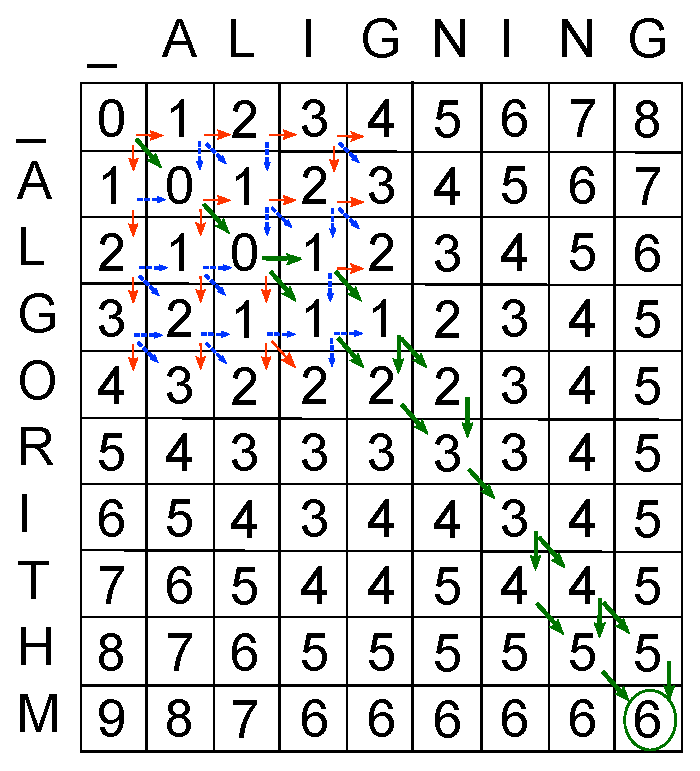
\includegraphics[scale=0.5] {img-align/edit-distance.eps}
%		\label{edit-distance}
%	}
%	\hspace*{0.5cm}
%	\subfigure[Resulting 9 optimal alignments - each part from the left concatenated with a right part. All the alignments have the last I's aligned, and there are 3 possible variations before and after the I's.] {
%		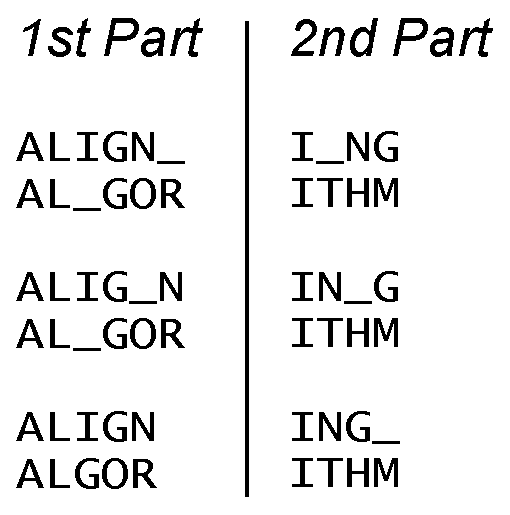
\includegraphics[scale=0.5] {img-align/alignments.eps}
%		\label{alignments}
%	}
%	%\caption{A figure example.}
%	%\label{fig:rmain figure}
%\end{figure}




%Edit distance of Damerau
%There is however a main limitation of Levenshtein's metric - it does not consider as a single 'edit operation' the transposition of elements. To face this problem, Damerau in 1964 \cite{damerau} proposed a new metric, with the 3 edit operations of Levenshtein and a new 4th operation - switching of two consecutive symbols. This is a very common source of misspellings, which was Damerau's motivation for the introduction of the new distance metric. The Levenshtein metric with Damerau's improvement is known as Levenshtein-Damerau Distance.




%%%%%%%%%%%%%%%%%%%%%%%%%%%%%%%%%%%%%%%%%%%%%%%%%%%%%%%%%%%%%%%%%%%%%%%
%%%%%%%%%%%%%%%%%%%%%%%%%%%%%%%%%%%%%%%%%%%%%%%%%%%%%%%%%%%%%%%%%%%%%%%

\subsection{\ac{NW} Algorithm for Global Alignment}

In 1970 \cite{needlemanwunsch} Needleman and Wunsch adapted the Levenshtein metric to use in the field of biological alignment. The \ac{NW} algorithm is mostly similar to the later Wagner and Fischer algorithm, with two differences introduced to improve its biological meaning:

	- Gaps are considered a single mutational event. A single "gap opening" penalty is weighted each time the alignment may evolve from a continuous region to a gap;

	- Each substitution may have a different real-world occurrence probability, and hence it should have a different weight. These probabilities were later measured and tabulated (see \sref{Substitution Scoring matrices}).

The resulting score of a global alignment, like that of a levenshtein edit distance, is given by the score of the last cell (which is the score of the complete path between the start of both sequences and their end). The function used for each cell may be the maximum or the minimum of previous cells.

Needleman and Wunsch's original metric for single gaps, and Sellers' similar method \cite{smith1981comparative}, were later extended by Waterman in 1976 \cite{waterman1976some} to support an arbitrary number of deletions/insertions and more complex gap cost models. Since then, all global alignment metrics and algorithms based on edit distances used for biological alignment are referred to as Needleman-Wunsch's.

Any type of function can be used for gap scoring, tough the function used has a great impact on the algorithm's complexity. If a linear cost function is used, each cell's value can be computed by inspecting only its direct ascendants (horizontal, vertical and diagonal). However, when using a non-linear cost function, such as an affine function with an initial gap opening constant penalty, this is not the case. Given the complex behavior of these functions, each value cannot be completely inferred from the previous discrete value. The contribution of a gap sequence may 'skip' some cells (usually the first) because the diagonal value presents a better option; and still be chosen for later cells, due to the function's amortized behavior (see \autoref{nw-complex-cost-models}). This means that, in order to compute each cell, the contributions of all the previous cells have to be considered and computed, and hence the algorithm's complexity rises from $O(n \times  m)$ to $O(n \times m \times max(n,m))$. 

\begin{figure}[htb!]
\centering
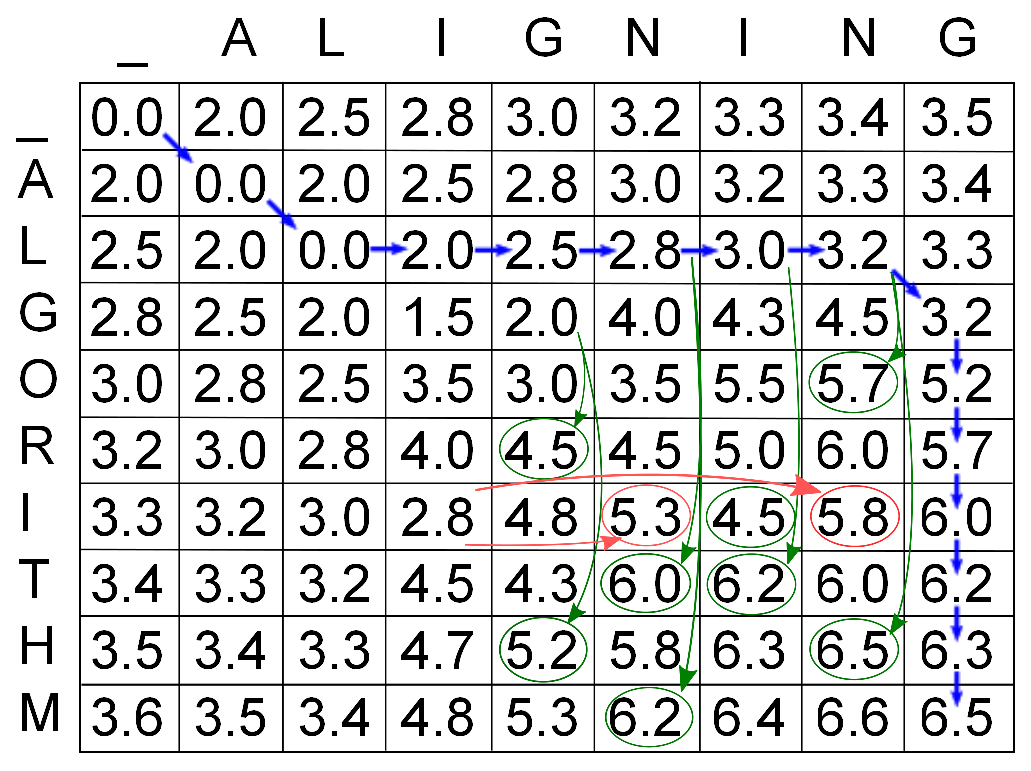
\includegraphics[scale=0.6]{img-align/nw-complex-cost-models.eps}
\caption[Needleman-Wunsch alignment] {Needleman-Wunsch matrix with a logarithmic gap model ($GapCost = 2 + 0.5 \times log_2(\#gaps)$, Match 0, Mismatch 1.5). Red and green arrows show the chosen non-continuous gaps (i.e. that are only chosen in later cells). The optimal alignment is traced in blue bold lines.}
\label{nw-complex-cost-models}
\end{figure}



\subsection{\ac{SW} Algorithm for Local Alignment}
\label{Smith-Waterman algorithm for Local Alignment}

Despite the good results of the \ac{NW} algorithm, most of the time molecular biologists do not want a global alignment. A global alignment forces all the sequences to be aligned - one way or the other. This means that, if there are regions with high similarity and regions with high divergence, the overall result would be average, or even bad. The interesting regions cannot be identified and extracted from the complete alignment. Moreover, global alignments always force the inclusion of gaps on the alignment fringes.

To tackle these limitations of global alignment, Smith and Waterman in 1981 \cite{smithwaterman} extended the previous algorithms with the possibility of "alignment restart", thus creating the first algorithm to compute local alignments (in \autoref{smith-waterman}). The \ac{SW} algorithm is similar to \ac{NW}'s and Sellers', with the differences:

	- Each cell value is maximized with 0. This mechanism causes a 'restarting' in the alignment path. Naturally, this requires the penalties to be negative and the match scores positive.

	- The maximum score may be obtained from any cell of of the matrix, instead of only the last one. Each cell holds the score for the optimal local alignment that ends in that cell.

	- To compute the gap cost, only those previous cells before the first zero (when followed backwards from the current cell) need to be inspected. All more distant previous cells cannot lead to a positive gap score.

\begin{figure}[htb!]
\centering
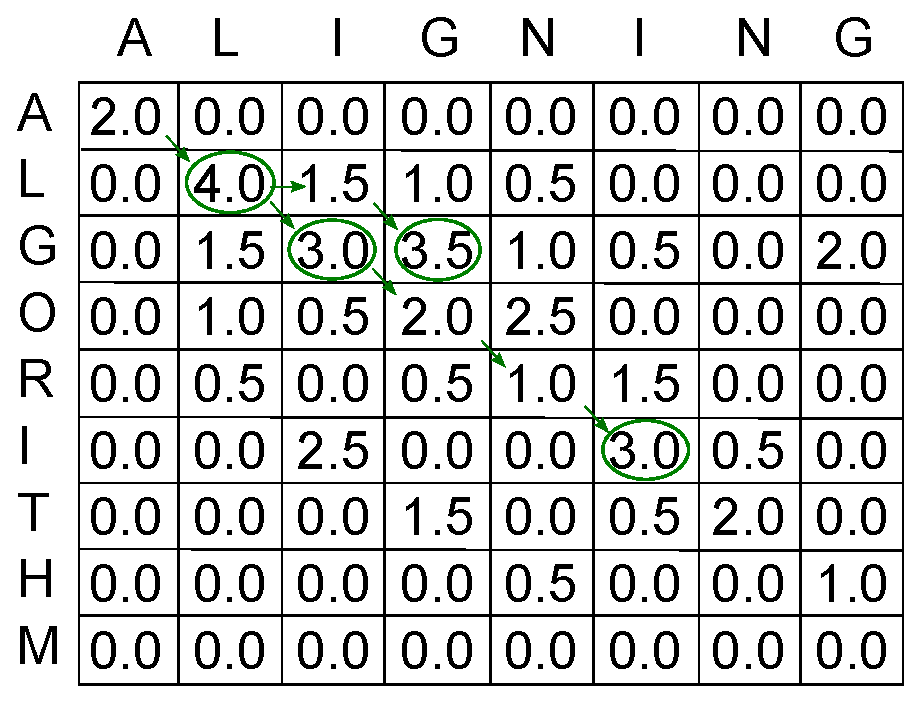
\includegraphics[scale=0.5]{img-align/smith-waterman.eps}
\caption[Smith-Waterman alignment] {Smith-waterman algorithm. $GapCost = -2 -0.5 \times (\#gaps)$, Match +2, Mismatch -1. The best alignments are shown and traced, with the maximum values circled.}
\label{smith-waterman}
\end{figure}


\subsection{Gotoh Algorithm}
\label{Gotoh algorithm}

These \ac{DP} algorithms are overly simple, and only a few optimizations have been found to reduce the required time and space lower bound. The quadratic time barrier cannot be lowered since they require that every cell in the $N \times M$ be computed. For arbitrary cost models, the complexity is even worse ($O(n^3)$). However, for some restricted cost models, a few improvements are possible.

Gotoh in 1982 \cite{gotoh} proposed a very important optimization for general \ac{DP} algorithms that use affine scoring functions. Such functions are actually one of the most suitable to biological sequences. Each gap opening is highly penalized, and all successive gaps have a reduced, linear cost, which models quite well the real-world occurrence of single mutational events, frequently responsible for inserting/deleting many elements at once.

Gotoh's algorithm is based upon the idea that the gap costs can also be modeled and computed in parallel, using Dynamic Programming, in separate matrices for vertical and horizontal gaps. Each cell in these two matrices hold the cost for a gap that ends in that cell.

These two matrices are computed based on their own dependencies and on the respective value in the main distance matrix (choosing the current main score 'restarts' the gap sequence, opening a new gap from the current cell). For the main matrix, the match/mismatch value is taken from its previous diagonal cell, and the gap contributions come from the same cell in the two twin matrices (i.e. the cost of a horizontal or vertical gap ending in that cell).

The gap matrices are usually named Q and P (after Gotoh), or E (horizontal) and F (vertical), while the main matrix is called D (distance matrix). The recursion relation can be formulated as follows:
\hspace{2 pc}  $$D_{m,n} = OP ( D_{m-1,n-1} + d(a_m,b_n) , E_{m,n} , F_{m,n} ) $$
Where OP may be Maximum or Minimum, and $d(a_m,b_n)$ is the match/mismatch score for the pair of elements $(a_m,b_n)$. E and F are both given by the same identical relation:
\hspace{2 pc}  $$E{m,n} = OP ( D_{m-1,n} + W_1 , E_{m-1,n} + W_{ext} ) 
\hspace{2 pc}  F{m,n} = OP ( D_{m,n-1} + W_1 , F_{m,n-1} + W_{ext} ) $$
$W_1$ is the gap cost function value for one gap, and $W_{ext}$ is the gap extension penalty, which is the slope of the affine cost function W. $W_i = W_{open} + i \times W_{ext}$. An example is presented in the associated figures.

Besides the reduced number of previous values that need be seen to compute each cell, Gotoh's improvement has another precious effect: the whole matrices are themselves not needed. They have to be computed but do not need to be stored, since only the last line column of diagonal of each one is used. As such, the algorithm can be very efficiently implemented on a computer, using only three of two arrays to store the intermediate cells. Gotoh's algorithm, therefore, reduces the time complexity to $O(N \times M)$ and the space complexity to O(min(n,m)).

One important note though, about reduced space requirements: gotoh's algorithm computes only the optimal score (or a set of scores, if they are saved separately). The alignment pattern itself cannot be extracted when this method is used, since no tracebacking data is stored.

\begin{figure}[htb!]
  \begin{minipage}{0.26\linewidth}
	\centering
	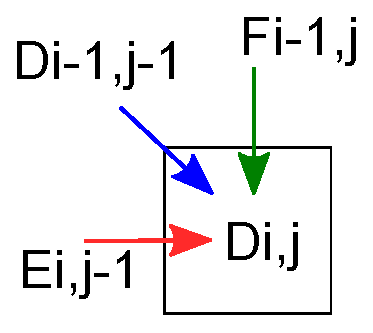
\includegraphics[scale=0.5]{img-align/nw-affine-gotoh-deps.eps}
	\caption[Gotoh's dependencies] {Dependencies for each cell of Gotoh's algorithm. Diagonal, horizontal and vertical.}
	\label{nw-affine-gotoh-deps}
  \end{minipage}
  \hspace{0.04\linewidth}
  \begin{minipage}{0.7\linewidth}
	\centering
	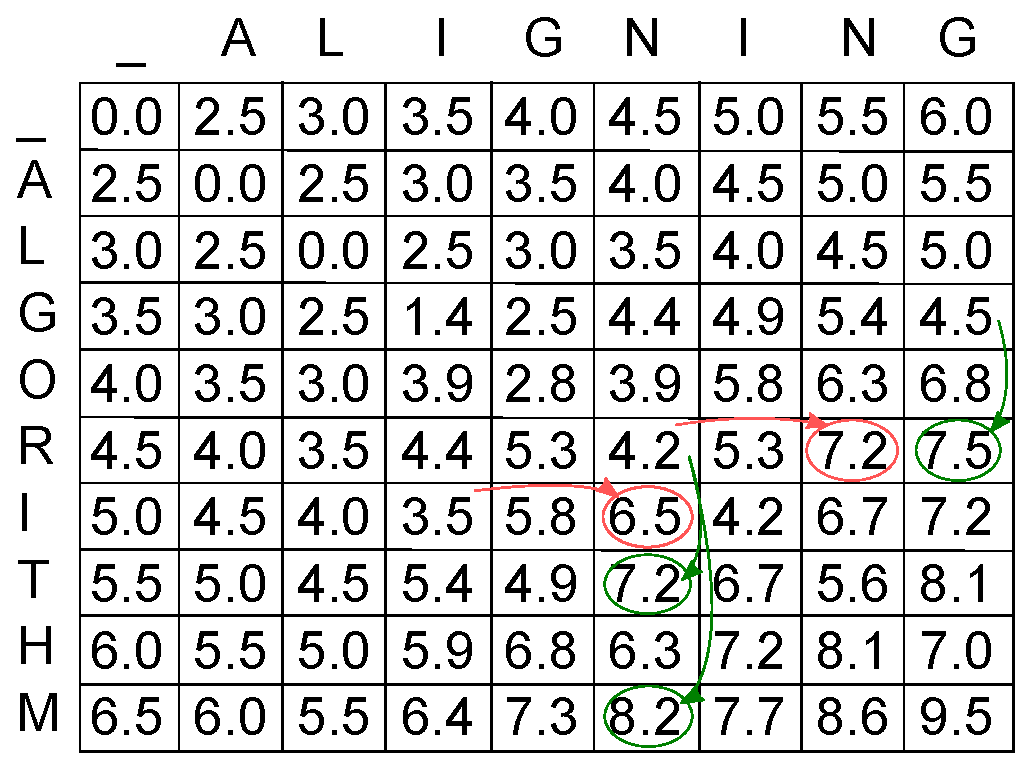
\includegraphics[scale=0.5]{img-align/nw-affine-gotoh-Dmat.eps}
	\caption[Gotoh's main matrix] {Gotoh's \ac{NW} algorithm D main matrix, with $GapCost = 2+0.5 \times (\#gaps)$, Match 0, Mismatch 1.4. Rightwards values in red come from the E matrix, and downwards green values from the F matrix.}
	\label{nw-affine-gotoh-Dmat}
  \end{minipage}
\end{figure} 


\begin{figure}[htb!]
 \begin{minipage}{0.48\linewidth}
	\centering
	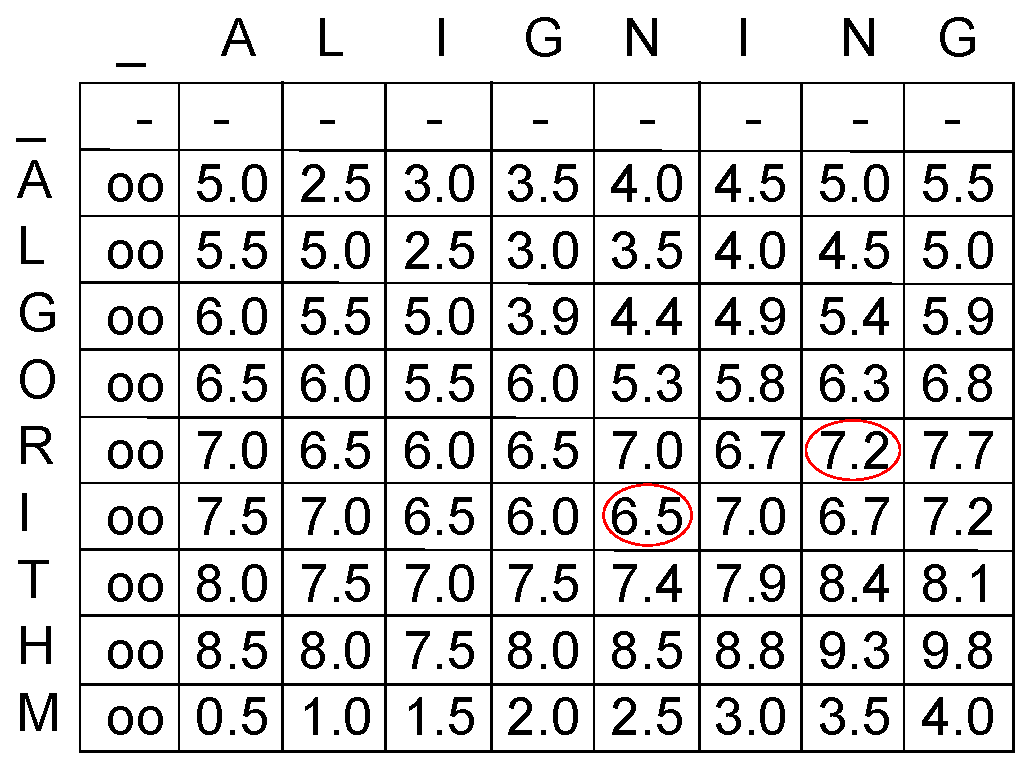
\includegraphics[scale=0.45]{img-align/nw-affine-gotoh-Emat.eps}
	\caption[Gotoh's E matrix] {Gotoh's left gaps (E) matrix. The values chosen for the main matrix are marked.}
	\label{nw-affine-gotoh-Emat}
  \end{minipage}
  \hspace{0.04\linewidth}
  \begin{minipage}{0.48\linewidth}
	\centering
	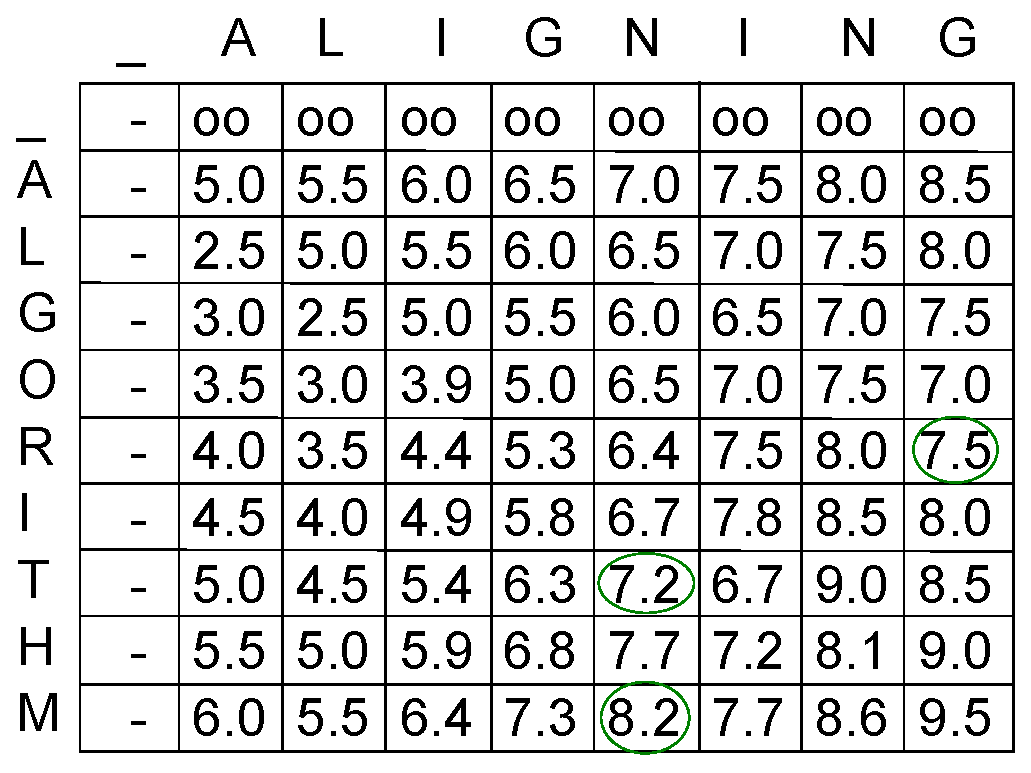
\includegraphics[scale=0.45]{img-align/nw-affine-gotoh-Fmat.eps}
	\caption[Gotoh's F matrix] {Gotoh's vertical gaps (F) matrix. The values chosen for the main matrix are marked.}
	\label{nw-affine-gotoh-Fmat}
  \end{minipage}
\end{figure} 



\subsection{SWAT optimization of the Smith-Waterman Algorithm}
\label{SWAT optimization}

%This improvement of the \ac{SW} algorithm is named after Green which first used it to great success in his 1993's SWAT program \cite{swat}. Pearson in 1991 had already implemented a similar optimization in the alignment kernel of FASTA, ssearch \cite{ssearch}.

For most sequences and typical scores, the D value in the Smith-Waterman algorithm remains at 0, or close by, in the majority of matrix cells (see \autoref{smith-waterman}). The E (horizontal) and F (vertical) dependencies can only affect D when the D value is higher (i.e. worse) than the weight of a single gap ($W_1 = W_{open} + 1 \times W_{ext}$). Such a penalty is usually chosen to be considerable costly, sometimes double the cost of a mismatch. Owing to that, only in relatively few cells are the E and F vectors able to affect the D cell value.

The SWAT optimization (\cite{swat},\cite{ssearch}) exploits this tendency. It consists of a relaxation in the required cells that need to be seen to evaluate the gap dependencies: all F and E cells lower than $W_1$ cannot contribute to the alignment, and neither can all cells before those, because they would offer a worse gap starting point. Therefore the previously presented zero-barrier may be extended to a $W_1$-barrier.

Using the original zero-barrier and this optimization, the cubic complexity of the \ac{SW} algorithm can be lowered in practice to $O(a \times n \times m)$, where '$a$' is some empirical constant. The Gotoh variant can also be greatly improved with these barriers, by ignoring the E and F values below the threshold.


%%%%%%%%%%%%%%%%%%%%%%%%%%%%%%%%%%%%%%%%%%%%%%%%%%%%%%%%%%%%%%%%%%%%%%%
%%%%%%%%%%%%%%%%%%%%%%%%%%%%%%%%%%%%%%%%%%%%%%%%%%%%%%%%%%%%%%%%%%%%%%%

\subsection{Substitution Scoring matrices}
\label{Substitution Scoring matrices}

Alignment algorithms operate on the special context of biological systems. Each sequence base (or residue) has a specific and distinct nature. Some are more frequent than others, some degenerate and mutate more easily, some are found more frequently in some regions. In particular, each symbol has a different probability of mutation into each other specific symbol. In order to accurately study and predict these dynamic biological events, the scoring system used to evaluate each sequence pair must take all this into account, and it must be constructed and trained with real biological data (i.e. mutations empirically observed in proteins and nucleic acids). These values were measured by Dayhoff in 1978 \cite{pam} to create PAM matrices, and by Henikoff in 1992 \cite{blosum} in the form of BLOSUM matrices, using a logarithmic scale. The two matrix types use opposite scoring schemes: PAMs were constructed from the observed mutations along a phylogenetic tree, whereas BLOSUMs measure the conserved regions. A lower PAM (fewer mutations) corresponds to a higher BLOSUM (more conservation), and vice versa.

An extension of the concept of substitution scores matrix is the \acp{PSSM}, also known as (Position Specific) Weight matrices, Frequency matrices or Profile matrices. These matrices count the number of occurrences of each symbol (line), for each sequence position (row). Employing \acp{PSSM} instead of simple substitution matrices has been proven to better model the sequences' homology. \cite{gribskov1987profile} \cite{henikoff1994position} \cite{rudnickipssms}



%%%%%%%%%%%%%%%%%%%%%%%%%%%%%%%%%%%%%%%%%%%%%%%%%%%%%%%%%%%%%%%%%%%%%%%
%%%%%%%%%%%%%%%%%%%%%%%%%%%%%%%%%%%%%%%%%%%%%%%%%%%%%%%%%%%%%%%%%%%%%%%
%%%%%%%%%%%%%%%%%%%%%%%%%%%%%%%%%%%%%%%%%%%%%%%%%%%%%%%%%%%%%%%%%%%%%%%
%%%%%%%%%%%%%%%%%%%%%%%%%%%%%%%%%%%%%%%%%%%%%%%%%%%%%%%%%%%%%%%%%%%%%%%







%%%%%%%%%%%%%%%%%%%%%%%%%%%%%%%%%%%%%%%%%%%%%%%%%%%%%%%%%%%%%%%%%%%%%%%%%%%%%%%%%%%%%%%%%%%%%%%%%%%%%%%
%%%%%%%%%%%%%%%%%%%%%%%%%%%%%%%%%%%%%%%%%%%%%%%%%%%%%%%%%%%%%%%%%%%%%%%%%%%%%%%%%%%%%%%%%%%%%%%%%%%%%%%
%%%%%%%%%%%%%%%%%%%%%%%%%%%%%%%%%%%%%%%%%%%%%%%%%%%%%%%%%%%%%%%%%%%%%%%%%%%%%%%%%%%%%%%%%%%%%%%%%%%%%%%
%%%%%%%%%%%%%%%%%%%%%%%%%%%%%%%%%%%%%%%%%%%%%%%%%%%%%%%%%%%%%%%%%%%%%%%%%%%%%%%%%%%%%%%%%%%%%%%%%%%%%%%

\section{Homology Search with Markov Models}

In this section, a different approach to sequence homology search will be described, an approach based on Hidden Markov Models. Despite the differen formulation of the problem, the  computation involved is very similar, and thus the algorithms and parallelization methods previusly analyzed, for the most part, can equally be used with Markov Models. 


\subsection{Markov Models}

In this section,  we will first introduce very briefly what are Markov Models.
A Markov Model is a probabilistic model of a system which enjoys the Markov property: the future states of the system depend entirely on the present state, and not on any previous states. A Hidden Markov Model (abbreviated HMM) is a Markov Model with unobserved states, so called 'hidden states'. In a HMM, the states may emit more than one possible token, according to a probability distribution. A HMM is therefore characterized by a number of unobserved states Q; a number of possible emission tokens T; a probability distribution of transitioning between the states Ft(q1,q2); and a probability distribution of emitting each token in each state Fe(q,w). The probability of some specific sequence of tokens being generated by a specific path of states $\pi$ is then given by:
$$P(x,\pi) = t_{0\pi_1} \prod\nolimits_{i=1}^L e_{\pi_i}(x_i) \times t_{\pi_i \pi_{i+1} }  $$

When using HMM, there are two tasks that are particularly important:
\begin{itemize}
	
	\item Decoding: Which path of states is the more likely to have generated a given token sequence, and what is the corresponding probability?
	This task is computed by the Viterbi Algorithm \cite{viterbi}, which progressively computes the most likely state to generate each new output symbol (i.e. token) , from the begin pseudo-state until reaching the end pseudo-state.	
	For each sucessive sequence symbol $x_i$, the Viterbi algorithm computes the recursive relations:
	$$ V_l(i) = e_l(x_i) \times max_k ( V_k (i-1) \times t_{kl} ) $$
	$$ Ptr_i(l) = argmax_k (V_k (i-1) \times t_{kl} ) $$	
	with $V_l(i)$ being the probability of being in state $l$, and emitting symbol $x_i$, and $Ptr_i(l)$ being the pointer to the chosen previous state.	
	To recover the most likely path, one must only traverse the computed pointers, $Ptr_i(l)$, in the reverse direction, from the end-state to begin-state.	
	
	\item Generation: What is the likelihood of a given sequence being generated by the model?

	To compute the likelihood probability, we need to sum the probabilities of all the possible generation paths. Since the number of possible paths is exponential, a more efficient method must be used. A solution is given by the Forward algorithm, which is similar to the Viterbi algorithm: a progressive sum of the probabilities of all previous state paths for each new token.

	For each sucessive sequence symbol $x_i$, the Forward procedure computes the following relation:
	$$ F_l(i) = e_l(x_i) \sum\limits_k F_k (i-1) \times t_{kl}  $$
	The final probability is calculated by summing the final probabilities of all the states:
	$$ F(x) = \sum\limits_k F_k (L) \times t_{k0}  $$
\end{itemize}

These two procedures can encounter value representation problems when implemented on a computer. Since they involve sucessive products of small probabilities, especially the Viterbi algorithm, the computed probalities quickly exceed the floating-point representation range of modern computers and go into underflow. This can be avoided by working in log-space, with logarithmic probabilities in every calculation, and the products turned into sums.

\label{log-transform}
The Logarithmic transformation poses a problem in the Forward algorithm: the log of a sum of two arguments is not easily computed from the logs of the arguments. The exact value is given by  $ \tilde{r} = log (exp(\tilde{a_1}) + exp(\tilde{a_2})) $, which can be written as $ \tilde{ r } = \tilde{a_1} + log (1 + exp(\tilde{a_2} - \tilde{a_1}))$. However, the function $log (1 + exp(\tilde{a_2} - \tilde{a_1}))$ can be approximated by interpolation from a table with a reasonably small size. \cite{hmmsbook}.

HMM have been used quite successfully for the past decades for various applications of statistical modeling and machine learning \cite{hmms-speech}.




\subsection{Alignment Profiles}

Until now, we have been looking at the homology search problem through the process of single alignment of one sequence against another.
In real applications however, namely for searching homologs (i.e. similar sequences) in a databse, we are looking for sequences that belong to a certain family or have a high similarity to a given group of sequences. Therefore, it is oftentimes more useful to search and compare the database against a group of sequences instead of a single query.

%\begin{figure}[htb!]
%  \begin{center}
%    \resizebox*{0.5\columnwidth}{!}{ 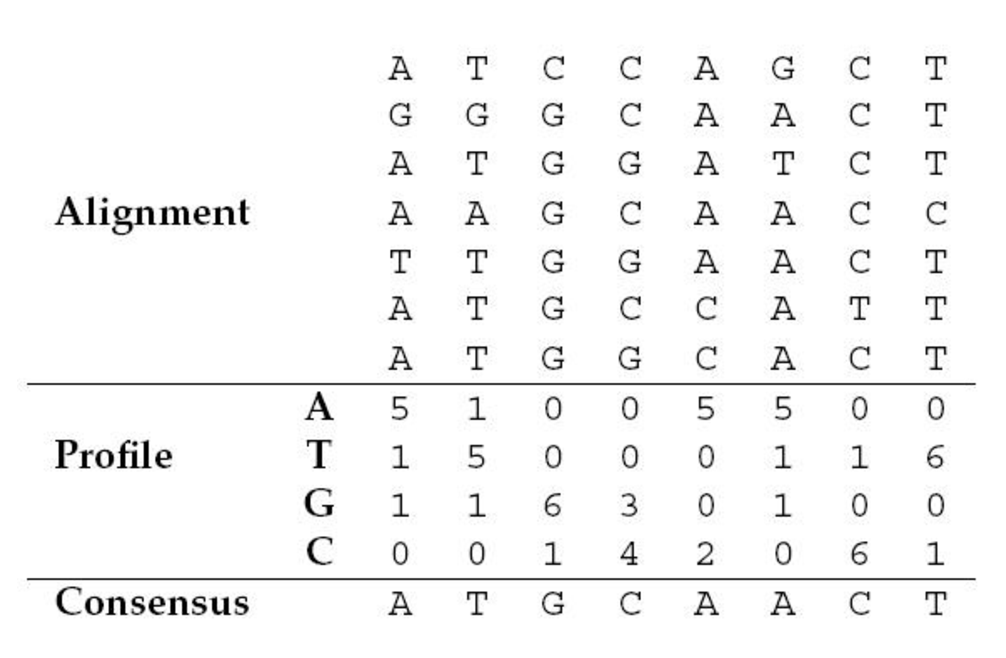
\includegraphics{img-align/consensus-profile.eps} }
%    \caption[Consensus Profile] {Example of a Consensus Profile derived from a multiple alignment of a family of similar sequences.}
%    \label{consensus-profile}
%  \end{center}
%\end{figure}

\begin{table}[h!]
\centering
\caption[Consensus Profile example] {Example of a Consensus Profile derived from a multiple alignment of a family of similar sequences.}
\label{consensus-profile}

\begin{tabular}{cccccccccc}
\multirow{6}{*}{\textbf{Alignment}} &  & A & T & C & C & A & G & C & T \\
&  & G & G & G & C & A & A & C & T \\
&  & A & T & G & G & A & T & C & T \\
&  & A & A & G & C & A & A & C & C \\
&  & A & T & G & C & C & A & T & T \\
&  & A & T & G & G & C & A & C & T \\
\hline
\multirow{4}{*}{\textbf{Profile }} & \textbf{A} & 5 & 1 & 0 & 0 & 5 & 5 & 0 & 0 \\
& \textbf{C} & 0 & 0 & 1 & 4 & 2 & 0 & 6 & 1 \\
& \textbf{G} & 1 & 1 & 6 & 3 & 0 & 1 & 0 & 0 \\
& \textbf{T} & 1 & 5 & 0 & 0 & 0 & 1 & 1 & 6 \\
\hline
\textbf{Consensus} &  & A & T & G & C & A & A & C & T \\
\end{tabular}
\end{table}

Profiles provide a more flexible way to identify homologs of a certain family, by highlighting the family's common features, and downplaying the divergences between the family's sequences. There are many ways to generate profiles, but most involve an initial multiple alignment of the sequences, followed by a probabilistic breakdown of the elements (residues or base-pairs) present in each position.

Profiles can thus effectively model a whole sequence family. This allows for a more efficient homology search: instead of comparing a query to each sequence in the family, the query can be compared to the Profile alone, greatly reducing the involved computational cost. Besides, a Profile gives a more correct representation of the defining characteristics of a family, by weighing the elements in proportion to their actual frequency (and thus importance) in the underlying family.



\subsection{Profile Markov Models}

A promising and widely used type of Profile constructs are Hidden Markov Models \cite{hmms}. 

Hidden Markov Models can be used to statistically model the distribution of sequence elements in a Profile, capturing the probability of each element in each position as the emission probability of tokens in each state. In such a model, each model state represents one position of the family consensus.
These Profile HMMs are then used to search a sequence database, by computing the probability of each database sequence being generated by the query model.

HMMs may also be used to find distant homologs by iteratively building and refining a model that describes them (such as in the SAM tool, \cite{sam}). In such an application, we start with an empty model. Iteratively,  each new sequence is aligned against the model, and that alignment is used to add the sequence to the multiple alignment of sequences that underlie the model. Finally the model is re-parametrized with the new multiple alignment.

Krogh and Haussler in 1994 \cite{krogh1994} developed a straightforward generalized profile Hidden Markov Model for homology searches, that emulate the results of a optimal alignment algorithm. The model is composed by three different types of states, respectively for matches/mismatches, insertions and deletions.

\begin{figure}[htb!]
	\begin{minipage}{0.48\linewidth}
		\centering
		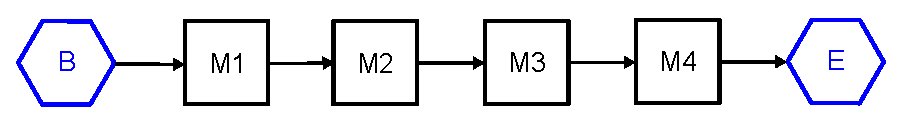
\includegraphics[scale=0.5]{img-hmm/model-construction-matches.eps}
		\caption[HMM for ungapped global alignment] {Example of a HMM composed solely of match states, allowing for ungapped global alignment.}
		\label{model-construction-matches}
	\end{minipage}
	\hspace{0.04\linewidth}
	\begin{minipage}{0.48\linewidth}
		\centering
		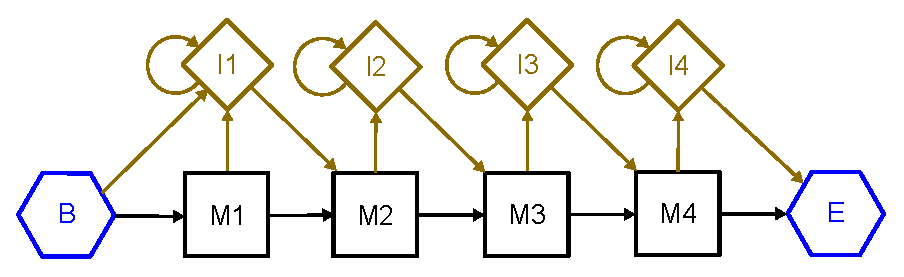
\includegraphics[scale=0.5]{img-hmm/model-construction-inserts.eps}
		\caption[HMM with Insert gaps] {Example of a HMM that allows arbitrary insertions. }
		\label{model-construction-inserts}
	\end{minipage}
\end{figure} 

The construction of the model is intuitive. First, a simple ungapped global alignment is modeled by a succession of match states, with a single string of transitions, as seen in \autoref{model-construction-matches}. These match states emit the alignment symbols, so they have a corresponding emission probability distribution, which is derived from the relative frequencies of symbols in the family's sequences. Since the symbols' frequencies vary in each position of the family's Profile, the emission distribution of the model, $e_{M_i}(x)$, will also be position-specific (similar to a \ac{PSSM}, see \sref{Substitution Scoring matrices}).

Our objective is to determine if a given sequence belongs to the model's family, so we have to discriminate the positive probability (sequence X generated by that model) against the negative probability (sequence X generated by some other random model). The negative probability is the background probability distribution, ${q_x}$., i.e., the probability of belonging to the standard random model. This is evaluated for the emission probabilities, in the form of log-odds ratios:

$ S(x) = log \frac{P(x|model)} {P(x|random)} = \sum\limits_{i=-1}^L log \frac{e_i{x_i}} {q_{x_i}} $

After having a model of match states for ungapped global alignment, we proceed to deal with gaps. It is possible to handle insertions (i.e., sections of the sequence $x$ that do not match the model) with an extra layer of states - insert states. An inserted region can occur at any point in the model, so we need to include an Insert state between each pair of match states. These new insert states must have a loop to allow for arbitrarily long inserted regions. A sketch of the resulting model with match and insert states is shown in \autoref{model-construction-inserts}.

These insert states also have an emission probability distribution $e_{I_i}(x)$, that represents the inserted symbols. This distribution however is arbitrary, it does not depend on the model, since these inserted elements are unknown to the model. To simplify the calculations, the insert emissions $e_{I_i}(x)$ are usually set to the background distribution ${q_x}$, resulting in a null odds-ratio contribution. The I $\rightarrow$ I model the gap-extend costs for non-matched symbols in the query sequence.

Lastly, deletions (portions of the profile not matched by the sequence) are added to the model, as forward jumps from each match state to every other suceeding match state. Each of the $N$ match states will have one average $\frac{N}{2}$ forward transitions. The basic idea is shown in \autoref{hmm-jumps1}. However, a topology with these forward jumps faces a cumbersome problem: the number of added transitions, $\frac{N^2}{2})$, is quite large, and can significantly slow down any algorithm. 

To circumvent the $\frac{N^2}{2})$ transitions, it is possible to develop an alternative topology that makes use of a third sucessive layer of silent 'jump states'. Silent states are those that do not emit any output symbol, but they may serve an important purpose in simplyfing a model. A forward jump is then achieved by sucessive transitions along the 'jump states' from one match state to the other, instead of a single transition between the two match states. A topology with jump states has the major advantage of using only a linear number of transitions ($N\times2$ new transitions) and new states ($N$ new states). An example of this topology is shown in \autoref{hmm-jumps2}.

\begin{figure}[htb!]
	\begin{minipage}{0.48\linewidth}
		\centering
		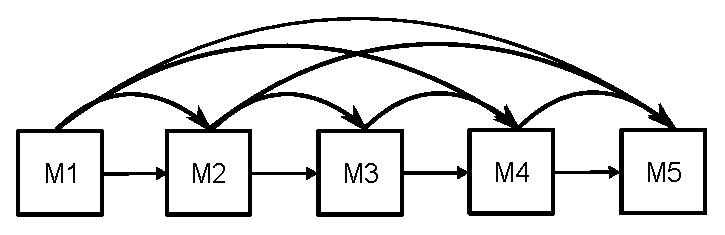
\includegraphics[scale=0.6]{img-hmm/hmm-jumps1.eps}
		\caption[HMM with Delete gaps] {Example of a HMM with a continuous sequence of states, and arbitrary jumps ahead.}
		\label{hmm-jumps1}
	\end{minipage}
	\hspace{0.04\linewidth}
	\begin{minipage}{0.48\linewidth}
		\centering
		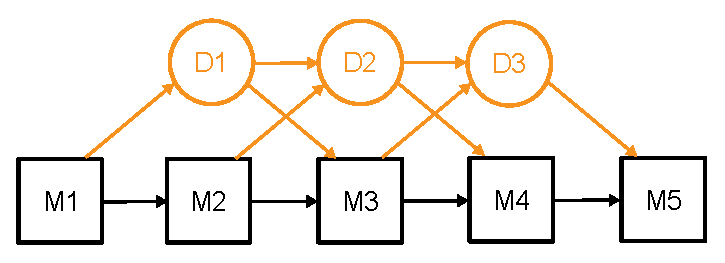
\includegraphics[scale=0.6]{img-hmm/hmm-jumps2.eps}
		\caption[HMM with Jump states] {Example of the previous HMM with the forward jump transitions converted to a layer of silent 'jump states'.}
		\label{hmm-jumps2}
	\end{minipage}
\end{figure} 

We can therefore use the 'jump states' as Delete states, where in each forward jump represents a region deleted from the profile model in the alignment. The D $\rightarrow$ D transitions thus correspond to gap-extend costs. Finally, the new layer of Delete states is added our previous model, which only had two layers, namely matches and inserts. Additional transitions from insert states to delete states, and vice-versa, can be included for the sake of correctness, although these transitions are usually very improbable and have a negligible effect. The final model for gapped global alignment, as proposed by Krogh and Haussler \cite{krogh1994}, can be seen in \autoref{krogh-haussler-model}. Krogh-Haussler's model is quite simple and intuitive, and has become the blueprint for later Profile HMMs \cite{sam}.

After having decided the structure of the HMM, it is necessary to parametrize it with the given family of sequences, namely to calculate from the data all the probability distributions required for the HMM. The parameterization of HMMs is a complex subject that falls outside the scope of this work (for this subject, see \cite{hmmsbook}). The Viterbi algorithm is also used for this purpose.

% STRESSAR que nao vamos abordar as formas de parametrizacao e os parametros usados no HMM
% Colunas com mais gaps que elementos sao modeladas por inserts

\begin{figure}[htb!]
  \begin{center}
    \resizebox*{1.0\columnwidth}{!}{ 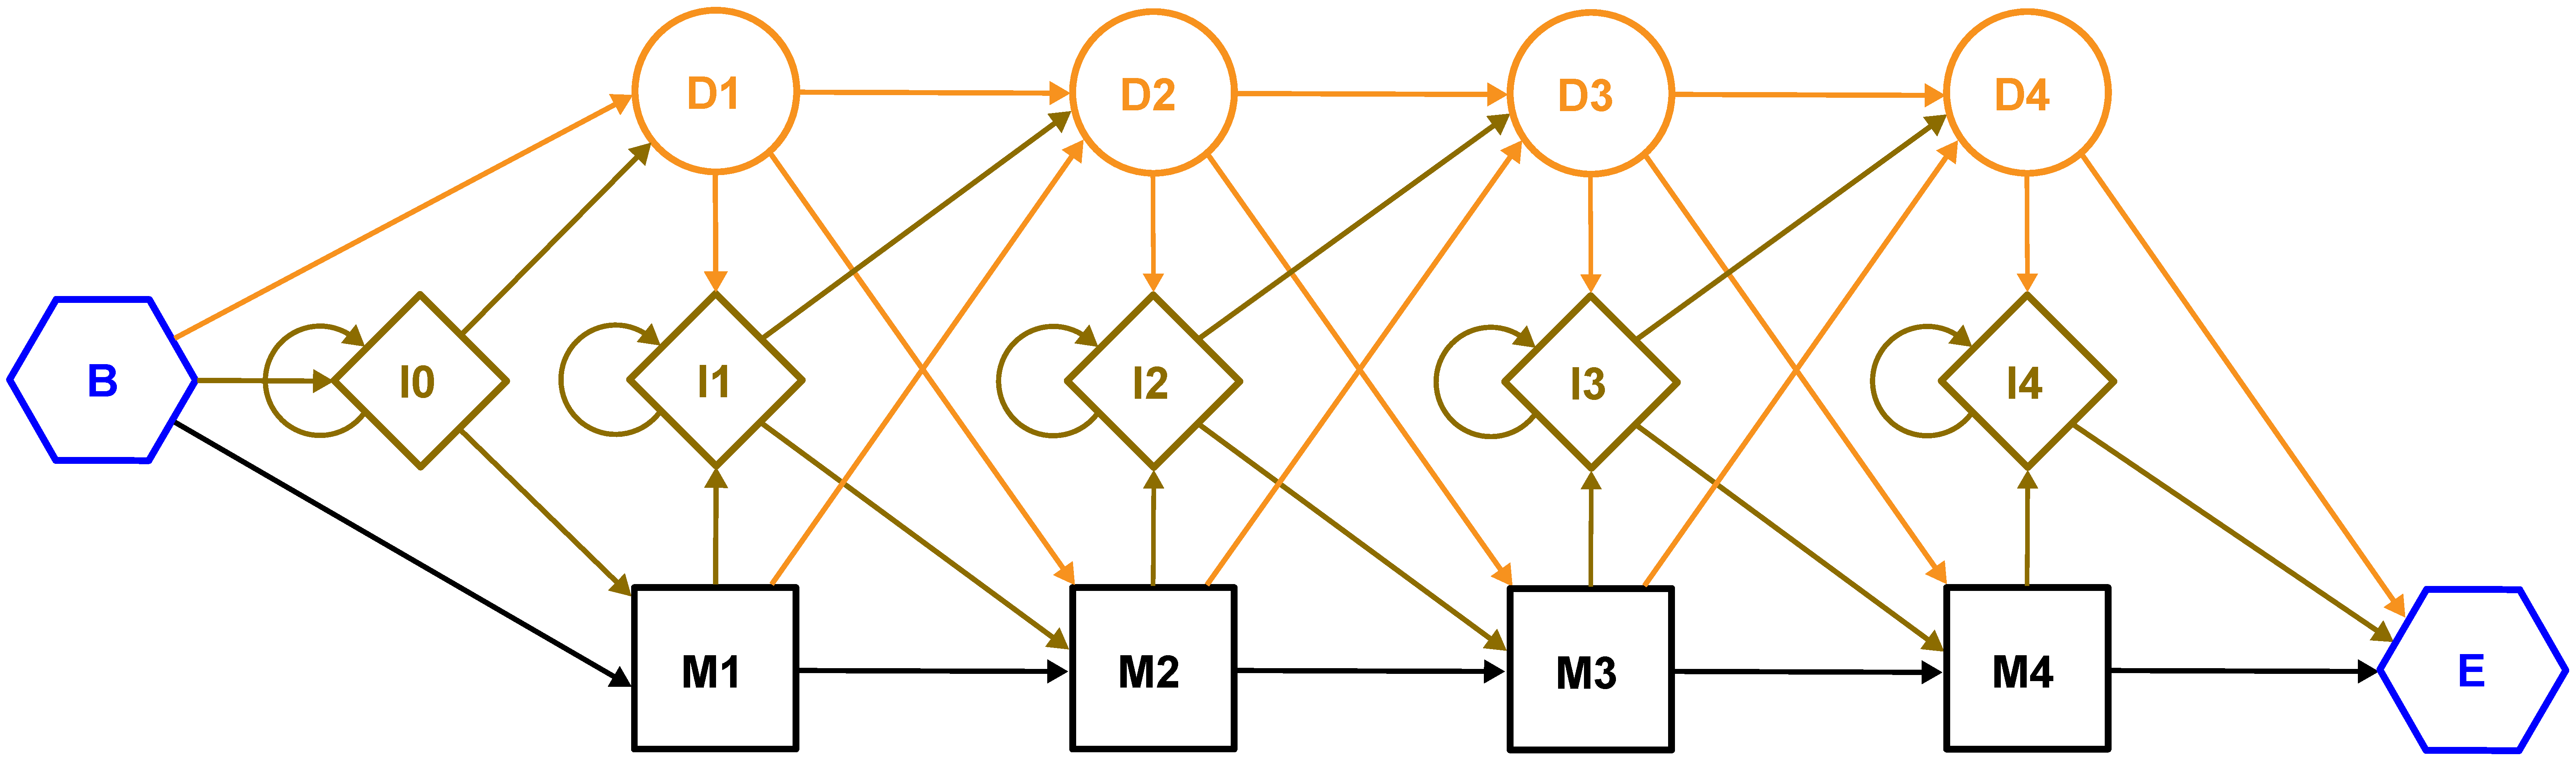
\includegraphics{img-hmm/krogh-haussler-model.eps} }
    \caption[HMM of Krogh-Haussler] {Krogh and Haussler' Hidden Markov Model for optimal gapped global alignment.}
    \label{krogh-haussler-model}
  \end{center}
\end{figure}





\subsection{Algorithms for global alignment Profile HMMs}

In a Profile HMM, the Viterbi algorithm gives the most likely path of states to generate the sequence, and the corresponding probability. It is therefore suitable for computing the alignment of the query sequence against the already multiple-aligned family's sequences (represented by the HMM). 

The Forward algorithm computes the overall likelihood of the sequence being generated by that model through any path, as opposed to a random model, by summing the probabilities of all possible paths. It is thus more suitable as a general similarity measure, indicating the likelihood of the query sequence belonging to the family.

For a global alignment Krogh-Haussler model, working in log-space, the Viterbi algorithm is expressed by the following \ac{DP} recurrence relations:
$$ V^M_j(i) = log \frac{e_{Mj}(x_i) }{q_{xi}} + Max  
		\begin{cases}
			V^M_{j-1} (i-1) + log\ t_{M_{j-1} M_j}  \\
			V^I_{j-1} (i-1) + log\ t_{I_{j-1} M_j}  \\
			V^D_{j-1} (i-1) + log\ t_{D_{j-1} M_j} 
		\end{cases} $$

$$ V^I_j(i) = log \frac{e_{Ij}(x_i) }{q_{xi}} + Max  
		\begin{cases}
			V^M_{j} (i-1) + log\ t_{M_{j} I_j}  \\
			V^I_{j} (i-1) + log\ t_{I_{j} I_j}  \\
			V^D_{j} (i-1) + log\ t_{D_{j} I_j}
		\end{cases} $$
$$V^D_j(i) = Max \begin{cases}
			V^M_{j-1} (i) + log\ t_{M_{j-1} D_j}  \\
			V^I_{j-1} (i) + log\ t_{I_{j-1} D_j}  \\
			V^D_{j-1} (i) + log\ t_{D_{j-1} D_j} 
		\end{cases} $$
$$ \\ $$

In regards to the Forward algorithms, for a global alignment model, working in log-space, we need to deal with following equations:
\begin{align*}
 F^M_j(i) = log \frac{e_{Mj}(x_i) }{q_{xi}} + log \;\;  
		[ \;\;  &t_{M_{j-1} M_j} \times exp \; (F^M_{j-1}(i-1))  \\ 
		+\;\;  &t_{I_{j-1} M_j}  \times exp \; (F^I_{j-1}(i-1))  \\
		+\;\;  &t_{D_{j-1} M_j} \times exp \; (F^D_{j-1}(i-1)) \;\; ] 
\end{align*}
\begin{align*}
 F^I_j(i) = log \frac{e_{Ij}(x_i) }{q_{xi}} + log \;\;  
		[ \;\;  &t_{M_{j} I_j} \times exp \; (F^M_{j}(i-1))  \\ 
		+\;\;  &t_{I_{j} I_j}  \times exp \; (F^I_{j}(i-1))  \\
		+\;\;  &t_{D_{j} I_j} \times exp \; (F^D_{j}(i-1)) \;\; ] 
\end{align*}
\begin{align*}
F^D_j(i) =  log \;\;[   \;\; &t_{M_{j} D_j} \times exp \; (F^M_{j-1}(i))  \\
			+\;\; &t_{I_{j} D_j} \times exp \; (F^I_{j-1}(i))  \\
			+\;\; &t_{D_{j} D_j} \times exp \; (F^D_{j_1}(i))  \;\; ]
\end{align*}



These equations are expensive to compute, given the logarithms and exponentials involved. An approximation can be devised through the use of interpolation, with lookup on a pre-computed $TabLog$ table (as previously explained in \sref{log-transform}), which yields the following pseudo-code:
\begin{align*}
 F^M_j(i) = log \frac{e_{Mj}(x_i) }{q_{xi}} + TabLog \;\;  
		[\;\; &log \; t_{M_{j-1} M_j} + F^M_{j-1}(i-1), \\
		 \;\;  TabLog \; [ \; &log \; t_{I_{j-1} M_j} + F^I_{j-1}(i-1)), \\
		 \;\;	&log \; t_{D_{j-1} M_j} + F^D_{j-1}(i-1) \;\; ] \;\; ]
\end{align*}
\begin{align*}
 F^I_j(i) = log \frac{e_{Ij}(x_i) }{q_{xi}} + TabLog \;\;  
		[\;\; &log \; t_{M_{j} M_j} + F^M_{j}(i-1), \\
		 \;\;  TabLog \; [ \; &log \; t_{I_{j} M_j} + F^I_{j}(i-1)), \\
		 \;\;	&log \; t_{D_{j} M_j} + F^D_{j}(i-1) \;\; ] \;\; ]
\end{align*}
\begin{align*}
F^D_j(i) = TabLog \;\; [ \; &log \; t_{M_{j} D_j} + F^M_{j-1}(i), \;\; \\
		&TabLog \; [	\; log \; t_{I_{j} D_j} + F^I_{j_1}(i),  
				\; log \; t_{D_{j} D_j} + F^D_{j_1}(i) ) \;\; ] \; ]
\end{align*}

The transition scores used are all in log-odds (i.e. $log \; t_{X_j Y_i }$).



\subsection{Simplification of the general Global Alignment HMM}

Some of terms may be removed from the Model. The D $\rightarrow$ I and I $\rightarrow$ D transitions have a negligible impact on the alignment, and therefore can also be removed. If the emission probabilities $e_{Ij}(x_i)$ are set to the background distribution, then the term $log \frac{e_{Ij}(x_i) }{q_{xi}}$ becomes null.

The simplified Viterbi equations in log-space are thus:

$$ V^M_j(i) = log \frac{e_{Mj}(x_i) }{q_{xi}} + Max  
		\begin{cases}
			V^M_{j-1} (i-1) + log\ t_{M_{j-1} M_j}  \\
			V^I_ {j-1} (i-1) + log\ t_{I_{j-1} M_j}  \\
			V^D_{j-1} (i-1) + log\ t_{D_{j-1} M_j} 
		\end{cases} $$

$$ V^I_j(i) = Max  
		\begin{cases}
			V^M_{j} (i-1) + log\ t_{M_{j} I_j}  \\
			V^I_{j} (i-1) + log\ t_{I_{j} I_j}
		\end{cases} $$

$$V^D_j(i) = Max \begin{cases}
			V^M_{j-1} (i) + log\ t_{M_{j-1} D_j}  \\
			V^D_{j-1} (i) + log\ t_{D_{j-1} D_j} 
		\end{cases} $$ \\

And the Forward equations in log-space, with the Interpolation approximation, become:
\begin{align*}
 F^M_j(i) = log \frac{e_{Mj}(x_i) }{q_{xi}} + TabLog \;\;  
		[\;\; &log\ t_{M_{j-1} M_j} + F^M_{j-1}(i-1), \\
		 \;\;  TabLog \; [ \; &log\ t_{I_{j-1} M_j} + F^I_{j-1}(i-1)), \\
		 \;\;	&log\ t_{D_{j-1} M_j} + F^D_{j-1}(i-1) \;\; ] \;\; ]
\end{align*}
\begin{align*}
&F^I_j(i) = TabLog	\;\; [	\;\; log\ t_{M_{j} I_j} + F^M_{j}(i-1), 
				\;\; log\ t_{I_{j} I_j} + F^I_{j}(i-1) ] \\
\\
&F^D_j(i) = TabLog \;\; [	\;\; log\ t_{M_{j} D_j} + F^M_{j-1}(i),
				\;\; log\ t_{D_{j} D_j} + F^D_{j_1}(i) ]
\\
\end{align*}




\subsection{Extension of Profile HMMs to Local Alignment}

A Profile HMM for global alignment may be converted to support local alignment as well, with the inclusion of some additional states. In essence, a local alignment constitutes a subregion of the query sequence that is aligned against a subregion of the model, with a significant score, flanked by two unmatched regions that include the rest of the query sequence and the rest of the model.

To capture a local alignment with a Profile HMM, one needs only to add these two 'flanking regions', for instance as sell-looping states with transitions from and to each match state (\cite{hmmsbook}). These 'flanking states' also emit tokens with a probability distribution, which we can set to the background random distribution to remove it from the computations. 

Therefore, the following specia-states are included:

\begin{itemize}

\item two flanking states connecting all normal states are added, the '$B$' state before and the '$E$' state after. These states have corresponding probability distributions for the array of possible transitions to or from normal states.

\item two self-looping flanking states, '$N$' before and '$C$' after. The self-looping states are characterized simply by a loop probability and a 'jump' probability out of the state.

\end{itemize}

An example of a Profile HMM to evaluate a single local alignment is shown in \autoref{model-local-unihit}.

\begin{figure}[htb!]
  \begin{center}
    \resizebox*{0.9\columnwidth}{!}{ 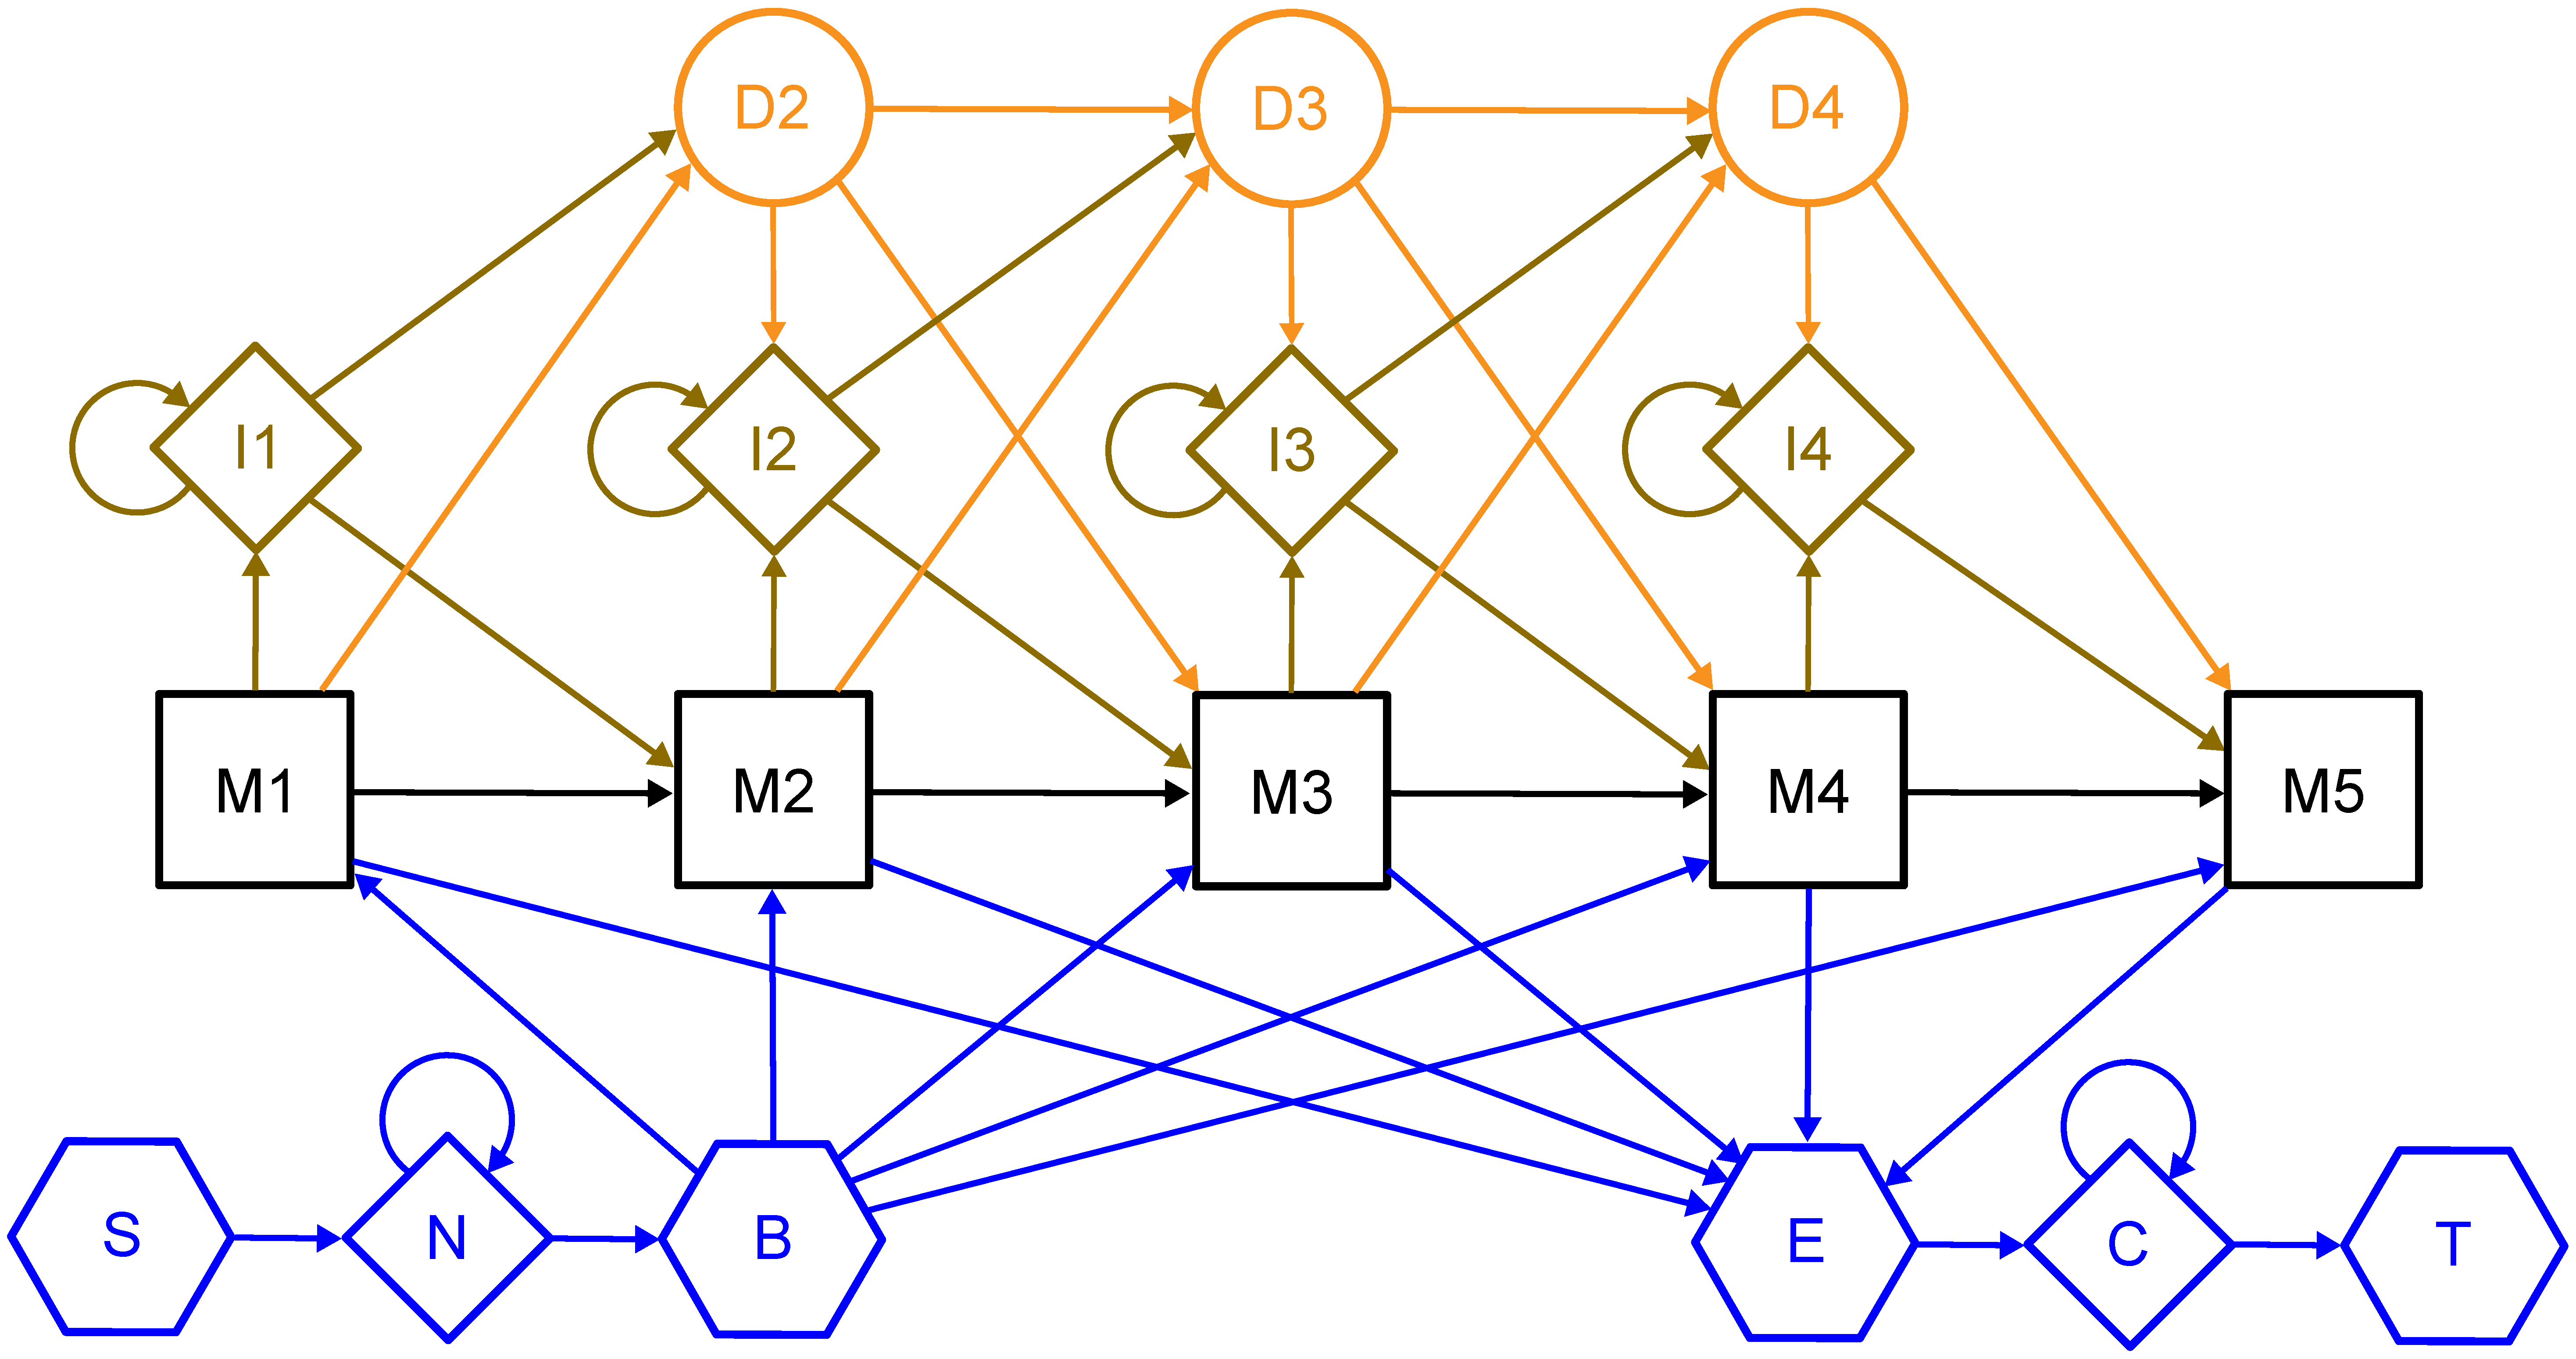
\includegraphics{img-hmm/model-local-unihit.eps} }
    \caption[HMM for unihit local alignment] {HMM for unihit local alignment (i.e. a single aligned region). }  
    \label{model-local-unihit}
  \end{center}
\end{figure}



\subsection{Extension of Profile HMMs to Multihit Alignments}

Up until now, it has only been discussed the case of \emph{unihit} evaluation with HMMs: only a single unbroken region, either the whole sequence and model (when in global alignment) or a subregion of the sequence and model (in the case of local alignment). It is also possible to use HMMs to match multiple regions, of both the sequence and the model. This is known as \emph{multihit} alignment mode, and it more closely resembles the classical alignment algorithms like Smith-Waterman. 

The previous HMMs can be extended to allow multihit alignments, by introducing another special state ('$J$'), connecting the $B$ and $E$ flanking states. This $J$ state requires only two parameters as well, a loop probability and a jump probability.

A multihit modeling capacity can be added to both global and local alignment HMMs. The \autoref{model-global-multihit} represents a HMM for multihit global alignment, while the more complex example for local alignment can be seen in \autoref{model-local-multihit}.

\begin{figure}[htb!]
  \begin{center}
    \resizebox*{1.0\columnwidth}{!}{ 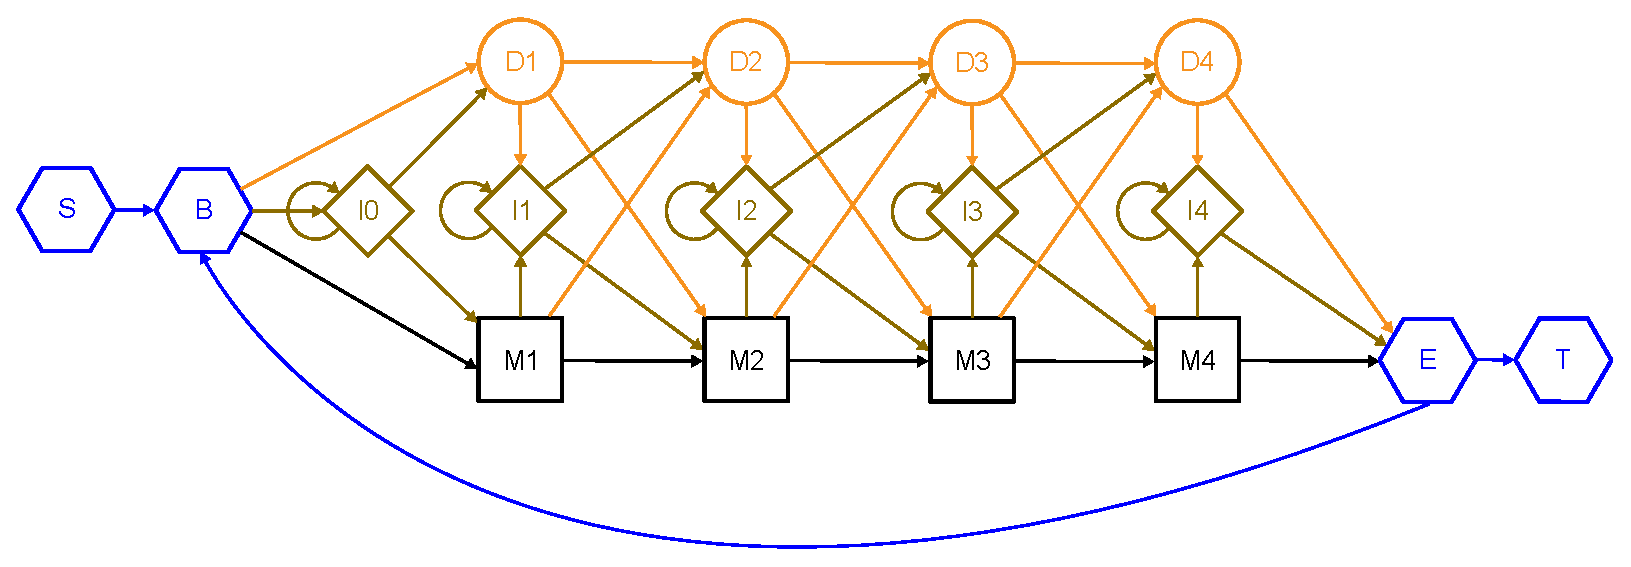
\includegraphics{img-hmm/model-global-multihit.eps} }
    \caption{HMM for multihit global alignment}  
    \label{model-global-multihit}
  \end{center}
\end{figure}


\begin{figure}[htb!]
  \begin{center}
    \resizebox*{0.9\columnwidth}{!}{ 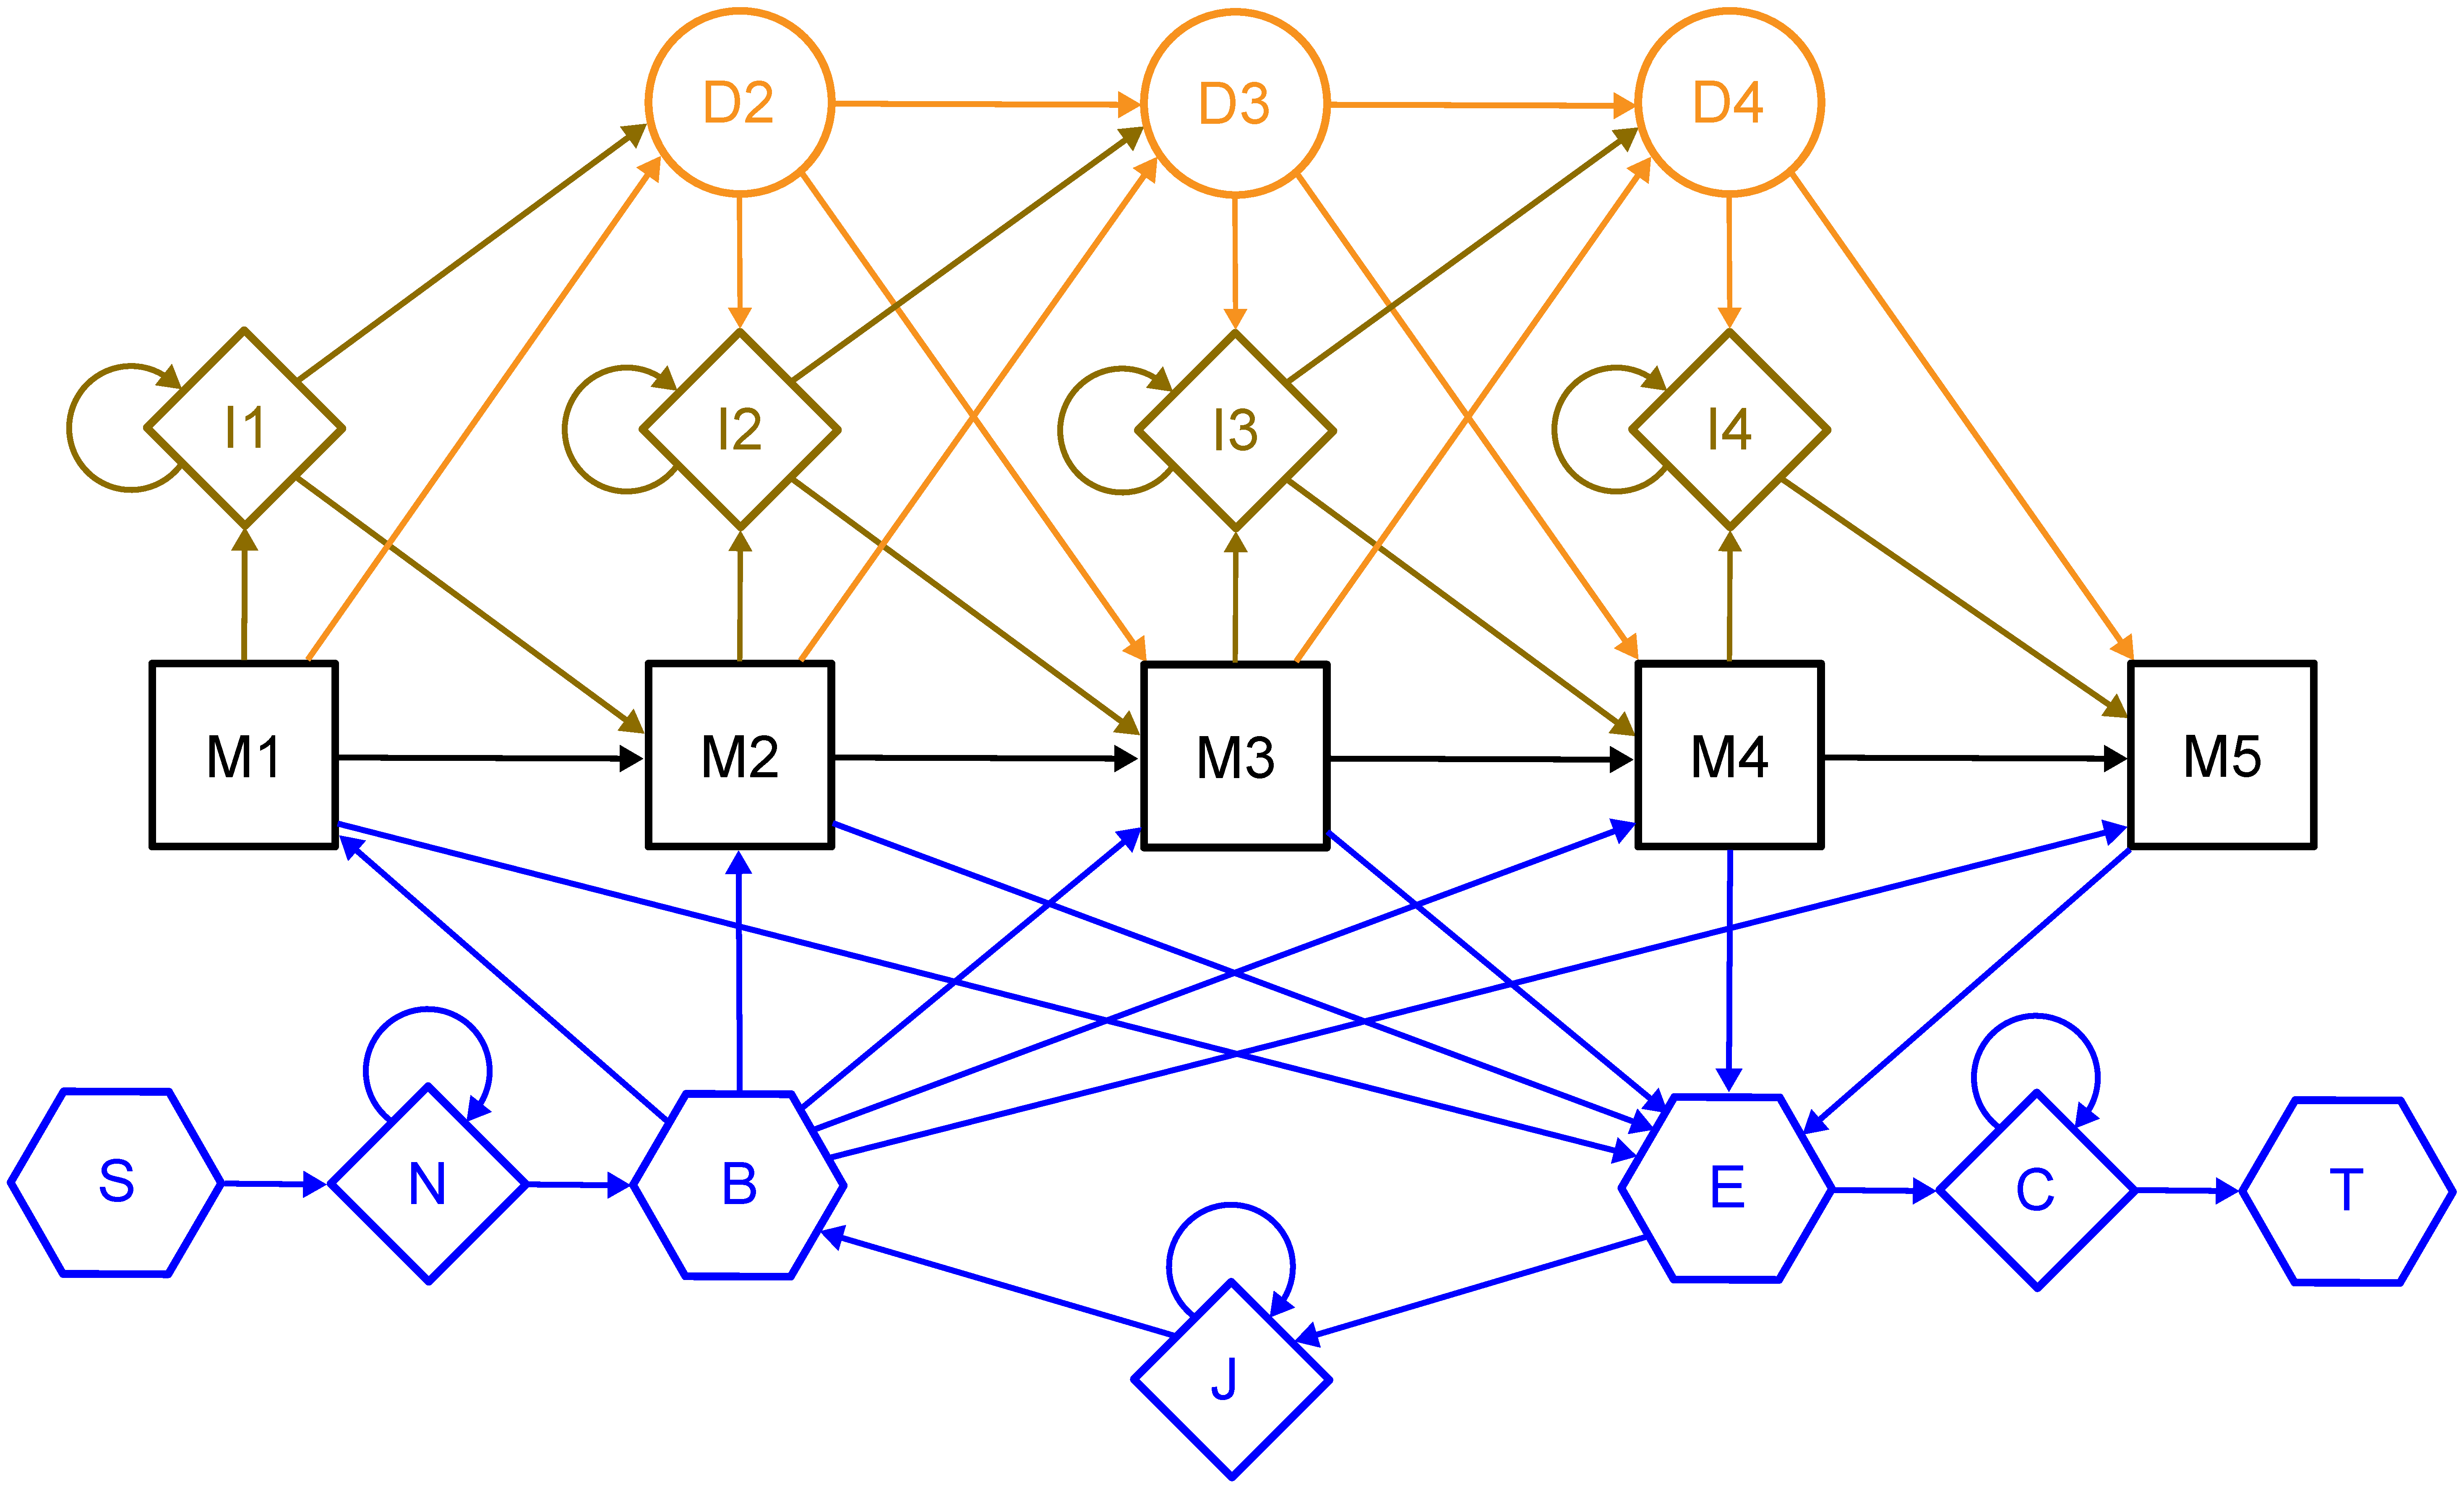
\includegraphics{img-hmm/model-local-multihit.eps} }
    \caption{HMM for multihit local alignment}  
    \label{model-local-multihit}
  \end{center}
\end{figure}

These multihit HMMs differ from the classical algorithms like Smith-Waterman and Needleman-Wunsch because the whole model is re-aligned against a new subregion of the sequence in each whole model loop. As a result, the same model region may be aligned multiple times to different sequence regions.

As for the algorithms to compute these multihit models, only the more interesting case of local alignment will be presented here.
The Viterbi algorithm for multihit local alignment can be computed by the pseudo-code in \cref{code-viterbi}.
The Forward algorithm for multihit local alignment model, with the additional special-states, is given by the pseudo-code in \cref{code-forward}.


%\cleardoublepage
\clearpage
 



%%%%%%%%%%%%%%%%%%%%%%%%%%%%%%%%%%%%%%%%%%%%%%%%%%%%%%%%%%%%%%%%%%%%%%%
%%%%%%%%%%%%%%%%%%%%%%%%%%%%%%%%%%%%%%%%%%%%%%%%%%%%%%%%%%%%%%%%%%%%%%%
